\documentclass[11pt,a4paper]{article}

\usepackage[utf8]{inputenc}
\usepackage[T1]{fontenc}
\usepackage[english]{babel}
\usepackage{lmodern}
\usepackage{microtype}
\usepackage[a4paper,margin=2.35cm]{geometry}
\usepackage{amsmath,amssymb}
\usepackage{booktabs,tabularx,multirow,threeparttable}
\usepackage{graphicx}
\usepackage{caption}
\usepackage{subcaption}
\usepackage{placeins}
\usepackage{float}
\usepackage{xcolor}
\usepackage{enumitem}
\usepackage{tikz}
\usetikzlibrary{arrows.meta,positioning,fit,shapes.geometric}
\usepackage[numbers,sort&compress]{natbib}
\usepackage{hyperref}
\usepackage[nameinlink,noabbrev]{cleveref}

\definecolor{cbrblue}{HTML}{4C78A8}
\definecolor{mmrred}{HTML}{E45756}
\definecolor{ontogreen}{HTML}{54A24B}
\hypersetup{
  colorlinks=true,
  linkcolor=black,
  citecolor=cbrblue,
  urlcolor=cbrblue,
  pdftitle={OntoCast and OPMAD for structured knowledge extraction from predictive-maintenance scientific literature},
  pdfauthor={}
}
\captionsetup{font=small,labelfont=bf}
\setlist{nosep,leftmargin=*}
\newcommand{\OPMAD}{\textsc{opmad}}
\newcommand{\OntoCast}{\textsc{OntoCast}}
\newcommand{\myCBR}{\textsc{myCBR}}
\newcommand{\MMR}{\textsc{mmr}}
\newcommand{\RDF}{\textsc{rdf}}
\newcommand{\ILD}{\textsc{ild}}

\title{\textbf{OntoCast and OPMAD for structured knowledge extraction from predictive-maintenance scientific literature}}
\author{}
\date{}

\begin{document}
\maketitle

\begin{abstract}
Scientific literature describes assets, signals, tasks, and models that can inform the conceptual design of predictive-maintenance systems, but transforming those texts into structured and auditable knowledge remains costly. A methodology is proposed to evaluate structured extraction with OPMAD-constrained \OntoCast{}: scientific text $\rightarrow$ RDF/Turtle facts $\rightarrow$ a 19-field schema $\rightarrow$ myCBR retrieval $\rightarrow$ a downstream maximal marginal relevance (MMR) reranking task. From 3,990 Scopus records published in 2025--2026, 2,768 were included and 1,822 PDFs were retrieved (1,821 unique documents). All retrieved documents yielded parseable artifacts and executable queries against 263 historical cases after RDF-star cleanup; the audits further quantified field coverage, defaults, SHACL conformance, traceability, and extractor-model effects. In the downstream task, with a pool of 15, top-5, and $\lambda=0.70$, mean intra-list dissimilarity increased from 0.4216 to 0.5265 and lists with repeated model signatures fell from 610 to 5; mean similarity decreased from 0.5563 to 0.5536 ($-0.48\%$). Max-sum and MAP-DPP comparators showed dependence on the diversity criterion, while candidate pools from 10 to 30 yielded a tunable trade-off. Intra-list dissimilarity reuses the similarity optimized by MMR and is not independent validation. As a methodological extension, text-level human annotation over frozen evidence packages is specified to compare \OntoCast{}--OPMAD with generic JSON extraction, LLM-generated schemas, and LLM-generated ontologies without auditing PDF-to-text conversion. The evidence supports executable interoperability and algorithmic ranking behavior; factual fidelity and decision utility are reserved for expert validation.

\vspace{0.5em}
\noindent\textbf{Keywords:} structured information extraction; ontologies; large language models; case-based reasoning; predictive maintenance; human evaluation.
\end{abstract}

\crefname{figure}{figure}{figures}
\crefname{table}{table}{tables}
\crefname{equation}{equation}{equations}
\Crefname{figure}{Figure}{Figures}
\Crefname{table}{Table}{Tables}
\Crefname{equation}{Equation}{Equations}

\section{Introduction}
\label{sec:intro}

Predictive maintenance organizes intervention decisions according to the condition and expected evolution of an asset. Its architectures combine acquisition, preprocessing, diagnosis, prognosis, and communication; each function can use knowledge-based, data-driven, physics-based, or multimodel configurations \citep{MonteroJimenez2020Survey}. During conceptual design, this breadth makes it difficult to select components and justify alternatives.

In operational terms, the problem studied is the following: an article describes an asset, signals, a task, and models; those facts must be converted into the attributes understood by a case-based reasoning (CBR) system, which returns historical experiences and candidate models. CBR reuses experiences through retrieval, reuse, revision, and retention \citep{Aamodt1994CBR,LopezDeMantaras2005CBR}; an ontology can provide vocabulary, structure, and semantic similarity \citep{Gruber1993Ontology,AmailefLu2013OntologyCBR,Qin2018OntologyCBR}. The existing infrastructure based on the \emph{Ontology model for Predictive Maintenance Architecture and Design} (\OPMAD{}) and on the \myCBR{} platform recommends predictive-maintenance models \citep{MonteroJimenez2021OPMADCBR,MunozHernandez2021OntologyCBR}, but it depends on manual incorporation and may return homogeneous solutions.

The study is motivated by three observations. First, large language models (LLMs) can extract graphs from text \citep{Pan2024LLMKG,Lairgi2024IText2KG}, but a parseable Resource Description Framework (RDF) file does not guarantee that the facts are correct, complete, or useful for a decision-support tool. Second, if those facts are to be used in an existing CBR system, they must be translated into a fixed attribute schema; information loss, default values, and disputable normalizations may appear in that step. Third, a CBR list ordered only by similarity may repeat very similar alternatives. Diversity is treated here as a separate downstream task: condensed nearest neighbour (CNN) methods modify the CBR memory \citep{MunozPena2025Diversity}; maximal marginal relevance (MMR) reversibly reorders a candidate set \citep{CarbonellGoldstein1998MMR}; and families such as explicit Query Aspect Diversification (xQuAD) or determinantal point processes (DPPs) represent other ways to cover intents or subsets \citep{Santos2010xQuAD,Gan2020DPP}.

The study does not propose a new ontology, CBR engine, or diversification algorithm. A methodology is proposed to convert scientific texts into structured knowledge with \OntoCast{} and \OPMAD{}, audit that conversion, and observe its effect on a downstream CBR task. Four questions are posed:

\begin{description}[style=nextline,leftmargin=1.5cm,labelwidth=1.2cm]
  \item[Q1.] To what extent does OPMAD-constrained \OntoCast{} produce a structured, traceable, and auditable representation of scientific articles on predictive maintenance?
  \item[Q2.] What part of that representation can be transformed into the 19-field CBR schema and into executable queries, and where do information loss or default values appear?
  \item[Q3.] What effect does the extracted representation have on a downstream task of retrieval and recommendation diversification, and how dependent is that effect on reranking criteria and parameters?
  \item[Q4.] How can the semantic fidelity of extractions be validated through human annotation and LLM comparators without conflating that validation with an audit of conversion from portable document format (PDF) to text?
\end{description}

The contribution is organized into six elements:

\begin{enumerate}[label=(\roman*)]
  \item a reproducible methodology to transform facts extracted with \OntoCast{} and \OPMAD{} into a 19-field schema compatible with CBR;
  \item a batch evaluation against a historical base of 263 cases, used as a downstream task and not as validation of factual truth;
  \item an MMR reranking layer and explicit comparators to analyze the trade-off between similarity and diversity without modifying the case base;
  \item audits of coverage, conformance with the Shapes Constraint Language (SHACL), default values, provenance, traceability, and differences between extraction models;
  \item paired analysis and cluster bootstrap over 1,821 queries, to avoid interpreting repeated rankings as independent evidence;
  \item reproducible artifacts and a text-level human annotation protocol over frozen evidence, designed to evaluate semantic fidelity without auditing PDF-to-text conversion.
\end{enumerate}

\section{Background and related work}
\label{sec:related}

\subsection{Ontologies and CBR in predictive maintenance}

An ontology formalizes shared concepts and relations \citep{Gruber1993Ontology,NoyMcGuinness2001Ontology101}. In CBR systems, this structure helps name attributes, organize cases, and calculate similarities that are more informed than a purely lexical comparison. Consequently, the integration between ontologies and CBR has been used in domains such as emergencies, tolerances, design, and process selection \citep{AmailefLu2013OntologyCBR,Qin2018OntologyCBR,RomeroBejarano2014CBRDesign,Mabkhot2019OntologyCBR}. Maintenance research also includes graphs intended to support decisions, for example by recommending plans through graph neural networks \citep{Xia2023MaintenanceKG}.

Within this line, \OPMAD{} offers a specialized vocabulary for articles, assets, variables, models, and predictive-maintenance functions. The \OPMAD{}--\myCBR{} infrastructure already integrates this terminology with a historical case base and similarity functions \citep{MonteroJimenez2021OPMADCBR,MunozHernandez2021OntologyCBR}. Therefore, the present work does not claim novelty in the ontology, the case base, or the CBR engine. The addressed problem is different: how to populate and evaluate that representation from heterogeneous scientific literature and full text.

\subsection{Structured extraction with language models}

Language models have been used to build and complete graphs, align vocabularies, and generate structured representations from text \citep{Pan2024LLMKG}. For example, iText2KG builds knowledge graphs incrementally \citep{Lairgi2024IText2KG}; other work guides the model with ontologies or automates mappings to RDF \citep{Mustafa2025OntologyGuided,Marketakis2026RDFMappings}. \OntoCast{} belongs to this family because it uses an ontology as a constraint to produce structured facts \citep{Belikov2025OntoCast}.

The difficulty does not end when a parseable graph is obtained. A graph may be well formed and still omit models, assign facts to a cited work, use overly generic labels, or generate values incompatible with a downstream application. Evaluation should therefore separate at least three levels: structural conformance, field coverage, and semantic fidelity with respect to the text. In this manuscript, structural conformance is checked with minimal SHACL shapes \citep{SHACL2017}; coverage and normalization are audited field by field; and semantic fidelity is prepared through human annotation over frozen textual evidence.

\subsection{Retrieval and diversity as a downstream task}

CBR retrieval is based on similarity, but a list of highly similar cases may be of limited use if it repeats equivalent solutions. The literature therefore distinguishes between relevance and diversity \citep{SmythMcClave2001Diversity,McSherry2002Diversity}, and recommender systems study complementary measures such as coverage, novelty, or serendipity \citep{KaminskasBridge2016BeyondAccuracy}. In this manuscript, CBR retrieval is not used as a test of factual truth; it is used as a downstream task to observe what happens when extracted facts are translated into queries.

There are several ways to introduce diversity. Modified CNN condenses or reorganizes the case memory \citep{MunozPena2025Diversity}. By contrast, MMR penalizes similarity to already selected elements and reorders a candidate set without modifying the case base \citep{CarbonellGoldstein1998MMR}. xQuAD explicitly represents search aspects or intents \citep{Santos2010xQuAD}, whereas DPPs favor diverse subsets through a determinant \citep{Gan2020DPP}. Because of this conceptual difference, reranking is interpreted here as a secondary analysis of downstream use, not as the main extraction contribution.

\begin{table}[H]
\centering
\caption{Positioning of the study with respect to nearby research families.}
\label{tab:positioning}
\footnotesize
\begin{tabularx}{\linewidth}{lXXX}
\toprule
Family & Typical question & Usual evidence & Role in this study \\
\midrule
Language models and graphs & Can text be structured as a graph? & triples, classes, or relations & coverage, traceability, and downstream use are also evaluated \\
Ontology--CBR & Does an ontology improve case retrieval? & similarity, competence, or utility & \OPMAD{}--\myCBR{} is reused as existing infrastructure \\
Maintenance graphs & Do they support decisions about assets? & performance in an industrial task & used as a conceptual reference, not as a predictor \\
Diversification & Does the retrieved list cover alternatives? & relevance and diversity & analyzed as a secondary task after extraction \\
\bottomrule
\end{tabularx}
\end{table}

\section{Materials and methods}
\label{sec:methods}

\subsection{Study design}

A computational pipeline-evaluation experiment was conducted. The unit of analysis was a unique scientific document with an associated extraction artifact. Each document followed the same chain: \OPMAD{}-constrained fact extraction, cleanup and conversion to the 19-field schema, normalization of the fields usable by \myCBR{}, and generation of a query against the historical base of 263 cases. In this way, each document produced a structured representation and a query comparable with the others.

The retrieval comparison was paired because the same query was evaluated under two conditions: (a) the top-5 returned directly by \myCBR{} ordered by similarity, used as the baseline; and (b) a top-5 reordered with MMR from the 15 most similar candidates. This design keeps extraction, the RDF--CBR bridge, the case base, and the query constant; only the rule that selects the final list from the candidate set changes. Therefore, the observed differences in similarity and diversity are interpreted as the effect of reranking, not as differences between documents or between extractions.

In addition to that downstream comparison, interoperability and traceability audits were conducted: coverage of the 19 fields, SHACL conformance, use of default values, normalization to the historical vocabulary, language model that generated each artifact, confidence of the PDF--facts link, active attributes in the CBR query, and sensitivity to reranking parameters. The study did not train a predictor, did not evaluate real industrial diagnosis or prognosis, and did not measure human utility. The factual fidelity of the extractions is delimited through the human annotation protocol described in \cref{sec:human-annotation}, but its results are not part of this computational experiment.

\subsection{Corpus and screening}

The corpus was built from English-language Scopus records published in 2025--2026. The search strategy combined terms for predictive maintenance, condition-based maintenance, prognosis and system health, remaining useful life estimation, condition monitoring, and fault prognosis. To reduce noise, reviews and ambiguous uses of frequent acronyms were excluded. Screening applied two simultaneous inclusion criteria: the article had to refer to a designed physical asset and had to have an explicit purpose of maintenance, inspection, diagnosis, prognosis, or condition-based decision making.

The selection flow separated three stages: bibliographic retrieval, thematic screening, and full-text availability. From 3,990 retrieved records, 2,768 met the inclusion criteria and 1,222 were excluded. For the included records, the PDF was retrieved through legal access routes whenever possible; 1,822 files were obtained, two of which corresponded to the same content, so the analysis uses 1,821 unique documents. The 946 included records without accessible PDF were not treated as extraction failures, but as a source of coverage bias: full-text availability varied by year and access mode. \Cref{fig:flow-corpus} summarizes the flow; the Scopus query, record-level screening decisions, and availability audit are documented in the supplement.

\begin{figure}[t]
\centering
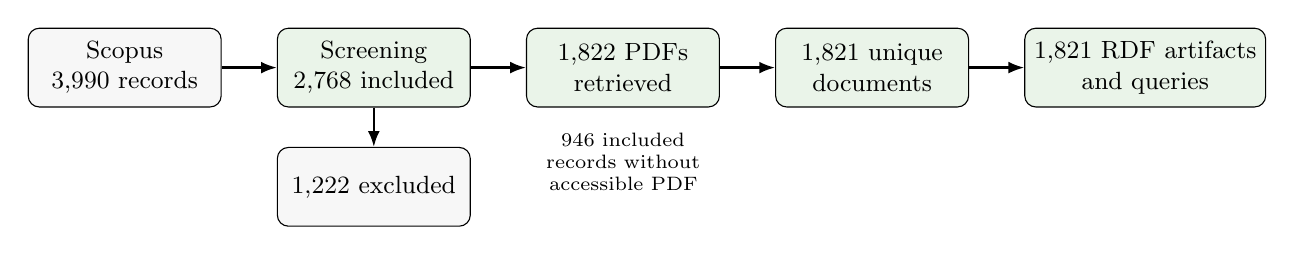
\begin{tikzpicture}[
  node distance=5mm and 7mm,
  box/.style={draw,rounded corners,align=center,minimum width=2.45cm,minimum height=1.0cm,fill=gray!6,font=\small},
  keep/.style={box,fill=ontogreen!12},
  arrow/.style={-{Latex[length=2mm]},thick}
]
\node[box] (scopus) {Scopus\\3,990 records};
\node[keep,right=of scopus] (screen) {Screening\\2,768 included};
\node[box,below=of screen] (excluded) {1,222 excluded};
\node[keep,right=of screen] (pdf) {1,822 PDFs\\retrieved};
\node[keep,right=of pdf] (unique) {1,821 unique\\documents};
\node[keep,right=of unique] (facts) {1,821 RDF artifacts\\and queries};
\draw[arrow] (scopus) -- (screen);
\draw[arrow] (screen) -- (pdf);
\draw[arrow] (pdf) -- (unique);
\draw[arrow] (unique) -- (facts);
\draw[arrow] (screen) -- (excluded);
\node[below=2mm of pdf,font=\scriptsize,align=center,text width=2.6cm] {946 included records without accessible PDF};
\end{tikzpicture}
\caption{Experimental corpus flow. The difference between 1,822 files and 1,821 documents is due to an exact duplicate, not to a missing extraction.}
\label{fig:flow-corpus}
\end{figure}

\subsection{OPMAD-constrained extraction}

Texts were processed in batches with GPT models using \OntoCast{} in fixed-ontology mode. Extraction used a self-contained \OPMAD{} seed (56 classes, 15 object properties, and two data properties) to constrain the vocabulary to articles, assets, variables, models, and maintenance functions. In this configuration, \OntoCast{} was not expected to create new classes or modify the ontology; for each document, it was expected to generate a Turtle file with facts compatible with \OPMAD{}.

Those Turtle files were the input to the RDF--CBR bridge described in the next subsection. Fact provenance was preserved for auditing, but it was not used as a CBR similarity or retrieval criterion.

\subsection{RDF--CBR bridge and normalization}

The \texttt{facts\_to\_csv.py} file acts as a bridge between RDF facts and the CBR schema. For each Turtle file, the bridge reads the graph, identifies entities by type, and retrieves their names through labels such as \texttt{schema:name} and \texttt{rdfs:label}. It then transforms the available information into a row validated by a 19-field Pydantic model. These fields group bibliographic metadata, maintenance task, asset, input signals or variables, preprocessing, model configuration and names, synchronization, failure modes, performance, and complementary notes.

When the graph contains no evidence for a field, the bridge uses explicit absence markers, such as \texttt{Not reported} or \texttt{Unknown synchronization}; some legacy numerical fields are completed with zero. These values make it possible to construct valid CSV files and executable queries, but they should not be interpreted as facts extracted from the text. For this reason, the audit distinguishes between informative values, default values, and automatically generated generic labels.

Each document was processed independently. If a Turtle file contained more than one possible case, one case was selected deterministically to avoid duplicating the document, although this rule does not always guarantee that the selected case corresponds to the source study. Before querying \myCBR{}, values were aligned with the historical vocabulary of the case base; unrecognized fields or default values without evidence were discarded or assigned zero weight. Structural conformance was checked with minimal SHACL shapes over titles, models, assets, and variables. This validation checks that the artifact has the expected structure, but it does not demonstrate factual accuracy with respect to the text.

\subsection{CBR retrieval}

The normalized queries were executed against the historical \myCBR{} base used in the \OPMAD{}--CBR infrastructure. This base contains 263 documented cases of model applications in predictive maintenance. To avoid inconsistencies between retrieval and subsequent analysis, the same version of the base was used both to query cases and to read the solution signatures used in diversity metrics. The extracted documents belong to 2025--2026, whereas the historical cases are earlier; therefore, the evaluation maintains a temporal separation between target literature and CBR memory.

Each query contains only the attributes that survived the bridge and normalization. \myCBR{} calculates global similarity from local similarities for task, asset type and name, synchronization, modality, input variables, and year. The task uses ontological relations, the asset name is compared with Levenshtein distance, and the input variables are treated as sets; other attributes use symbolic tables inherited from the previous infrastructure \citep{Sanchez2012SemanticSimilarity,MonteroJimenez2021OPMADCBR}. Empty attributes do not contribute weight to the query, and values used only as absence markers were not treated as evidence.

The direct output of \myCBR{} was used as the baseline: the five most similar cases form the top-5 without diversification. For the diversity condition, a candidate set of 15 cases was first retrieved and then the reranking described in the next subsection was applied. The query year was fixed at 2026 to keep the recency function constant. As sensitivity controls, queries with different attribute subsets and alternative years were evaluated to identify which part of the ranking depended on task, asset, variables, or recency.

\subsection{MMR reranking}
\label{sec:mmr}

Reranking was added as a postprocess to CBR retrieval. Its goal is not to change the similarity calculated by \myCBR{} or to modify the case base, but to select a less redundant final list from an already retrieved candidate set. In practical terms, each query first produces a pool of similar cases; MMR then chooses a short list that balances two criteria: preserving cases relevant to the query and avoiding solutions that are too similar to one another.

To measure whether two recommendations are similar, a solution similarity, $s_{\mathrm{sol}}$, was defined. This function does not compare the problems described by the articles, but the solutions recommended by the CBR base. It combines four components: model approach, model type, model names, and preprocessing:
\begin{equation}
 s_{\mathrm{sol}}(x,y)=0.20s_{\mathrm{approach}}+0.25s_{\mathrm{type}}+0.40s_{\mathrm{models}}+0.15s_{\mathrm{prep}}.
 \label{eq:solution-sim}
\end{equation}
The greatest weight was assigned to model names because the diversification objective was to reduce lists with repeated modeling alternatives. Lexical matches were combined for approach and type; for models, a taxonomy of terms from the historical base was added; and exact match was used for preprocessing. When a recommendation lists several algorithms in the \texttt{Models} field, the model signature is interpreted as a normalized multivalue string, not as a single algorithm.

MMR selects elements greedily. The first \myCBR{} result is preserved in order not to alter the most similar recommendation. Then each new element is chosen by maximizing:
\begin{equation}
 x^{*}=\arg\max_{x\in R\setminus S}\left[\lambda\,\mathrm{rel}(x)-(1-\lambda)\max_{y\in S}s_{\mathrm{sol}}(x,y)\right],
 \label{eq:mmr}
\end{equation}
where $R$ is the candidate pool, $S$ is the already selected list, and $\mathrm{rel}(x)$ is the global similarity calculated by \myCBR{}. The parameter $\lambda$ controls the trade-off: high values prioritize CBR relevance and low values penalize redundancy between solutions more strongly. The main configuration used $\lambda=0.70$, pool 15, and top-5 output.

To check that the conclusions did not depend on a single parametrization, alternative values of $\lambda$, pool sizes, list sizes, and weights of $s_{\mathrm{sol}}$ were evaluated. MMR was also compared with rules that respond to different criteria: exact deduplication of model signatures, max-sum selection, and MAP-DPP. These comparators are not presented as new methods; they are used to show whether the observed reduction in redundancy is specific to MMR or to the chosen diversity objective.

\begin{figure}[H]
\centering
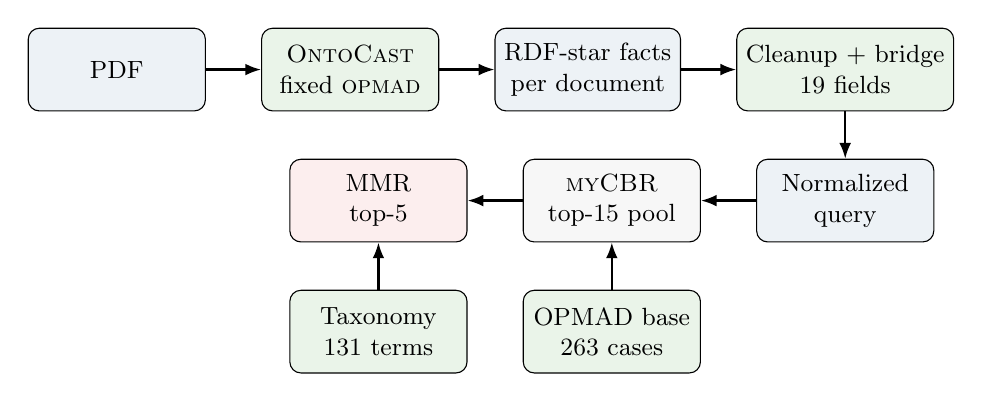
\begin{tikzpicture}[
  node distance=6mm and 7mm,
  proc/.style={draw,rounded corners,align=center,minimum width=2.25cm,minimum height=1.05cm,fill=gray!6,font=\small},
  data/.style={proc,fill=cbrblue!10},
  sem/.style={proc,fill=ontogreen!12},
  rank/.style={proc,fill=mmrred!10},
  arrow/.style={-{Latex[length=2mm]},thick}
]
\node[data] (pdf) {PDF};
\node[sem,right=of pdf] (cast) {\OntoCast{}\\fixed \OPMAD{}};
\node[data,right=of cast] (rdf) {RDF-star facts\\per document};
\node[sem,right=of rdf] (bridge) {Cleanup + bridge\\19 fields};
\node[data,below=of bridge] (query) {Normalized\\query};
\node[proc,left=of query] (cbr) {\myCBR{}\\top-15 pool};
\node[rank,left=of cbr] (mmr) {MMR\\top-5};
\node[sem,below=of cbr] (base) {OPMAD base\\263 cases};
\node[sem,below=of mmr] (tax) {Taxonomy\\131 terms};
\draw[arrow] (pdf) -- (cast);
\draw[arrow] (cast) -- (rdf);
\draw[arrow] (rdf) -- (bridge);
\draw[arrow] (bridge) -- (query);
\draw[arrow] (query) -- (cbr);
\draw[arrow] (cbr) -- (mmr);
\draw[arrow] (base) -- (cbr);
\draw[arrow] (tax) -- (mmr);
\end{tikzpicture}
\caption{Evaluated architecture. Reranking does not modify the case base or the CBR scores; it selects five recommendations from the pool of 15.}
\label{fig:architecture}
\end{figure}

\subsection{Text-level human annotation over frozen evidence}
\label{sec:human-annotation}

To evaluate extraction fidelity without turning the study into a PDF-to-text conversion audit, human validation was defined over frozen evidence packages. Each package contains an identifier, title, minimal metadata, and the text used as input by the extraction arms. PDFs remain as documentary references, but annotators should not verify whether the conversion faithfully reproduces the PDF; the evaluated construct is extraction from the available text.

The annotation unit is the document. Two independent specialists receive the packages in random order and without access to predictions, RDF facts, CBR queries, or rankings. For each document, they record a reference value for task, asset or case study, case type, model input, number and types of variables, preprocessing, approach, model types and names, synchronization, failure modes, performance indicators and values, title, and identifier. Scalar fields are annotated as a string, number, or \texttt{null}; multivalue fields as lists. When the frozen text does not contain sufficient evidence, the value is marked as absent and is not inferred from external knowledge.

In addition to the value, each annotator records a brief textual location within an evidence block and free notes. The evidence may be a section, converted page, heading, or short phrase within the package; its purpose is to make the decision auditable, not to measure OCR quality. After a calibration pilot outside the final estimate, disagreements are resolved by documented adjudication or by a third expert. The adjudicated file constitutes the reference standard for comparing OntoCast--\OPMAD{}, generic JSON extraction, LLM-generated schema, and LLM-generated ontology under abstract, section, and full-text views.

The metrics for this validation are calculated by document and field. For multivalue fields, normalized sets are compared and precision, recall, and F1 are reported; for scalar fields, normalized exact match and omission or commission errors are reported. A prediction with a value not supported by the reference standard counts as a false positive or operational hallucination; a value present in the reference standard and absent in the prediction counts as a false negative. Inter-annotator agreement is estimated before adjudication. This protocol is specified for a semantic-validation phase and does not introduce human results into the analyses reported below.

\subsection{Metrics and statistical analysis}

The metrics were organized into three groups. The first evaluates interoperability: number of documents with parseable artifacts, number of executable queries, non-default coverage of schema fields, and structural conformance through SHACL. These metrics indicate whether the chain produces computable objects, but they do not demonstrate that the values are correct with respect to the text.

The second group describes CBR retrieval before and after reranking. For each query, the similarity of the first result, the mean similarity of the top-5, the number of distinct model signatures, the presence of repeated signatures, order changes, and set changes were recorded. These measures make it possible to observe whether the postprocess modifies the final list and how much that modification costs in terms of CBR similarity.

The third group measures algorithmic diversity through intra-list dissimilarity. For a list $L$ of $k=5$ recommendations, the following was calculated:
\begin{equation}
 \ILD(L)=\frac{2}{k(k-1)}\sum_{i<j}\left[1-s_{\mathrm{sol}}(x_i,x_j)\right],\qquad k=5.
 \label{eq:ild}
\end{equation}
This metric uses the same solution similarity defined for MMR in \cref{eq:solution-sim}. It should therefore be interpreted as a measure aligned with the reranking objective, not as independent validation of utility, perceived novelty, or technical quality of the recommended models.

The main analysis was paired: for each document, the \myCBR{} top-5 list was compared with the top-5 list obtained after MMR. Mean differences and 95\% confidence intervals were reported through 20,000 bootstrap resamples. Because many queries may produce identical or very similar rankings, the bootstrap was repeated by clustering over normalized signatures and ranking patterns; this avoided treating duplicate rankings as fully independent evidence.

Sensitivity analyses evaluated changes in $\lambda$, pool size, list size, weights of the solution similarity, active query attributes, and year used by the recency function. Statistical tests are not interpreted as inference over a clinical or industrial population, but as stability of algorithmic behavior under the studied corpus. The human annotation described in \cref{sec:human-annotation} is reserved for measuring semantic fidelity of extraction and is not replaced by an LLM judge.

\FloatBarrier
\bibliographystyle{unsrtnat}
\bibliography{references}

\end{document}
